\documentclass{beamer}

\usepackage[latin1]{inputenc}
\usetheme{Dresden}
% Madrid, CambridgeUS
\title{Introduction to Ubuntu}
\author{Vikas Reddy}
\institute[Azri]{Azri Solutions}
\date{December 30, 2011}
\pgfdeclareimage[height=0.6cm]{logo}{azri-newlogo-small.png}
\logo{\pgfuseimage{logo}}

\begin{document}

 \begin{frame}
  \titlepage
 \end{frame}

 \begin{frame}{Outline}
  \tableofcontents
 \end{frame}

 \section{What is an open source software?}
 \begin{frame}{What is an open source software?}
  \begin{figure}
    
\includegraphics[width=4cm]{Images/opensource-logo}
  \end{figure}
  \begin{enumerate}
   \pause
   \item \textbf{freedom to run} the program, for any purpose.
   \pause
   \item \textbf{freedom to study} how the program works.
   \pause
   \item \textbf{freedom to redistribute} copies to help others.
   \pause
   \item \textbf{freedom to improve} the program, and release one's improvements to the public.
  \end{enumerate}
 \end{frame}

 \section{Why Ubuntu?}
 \begin{frame}{Why Ubuntu?}
  \begin{figure}
   
\includegraphics[width=2cm,height=2cm]{Images/cof_orange_hex1}
  \end{figure}
  \begin{itemize}
   \pause
   \item Free of cost
   \pause
   \item Liberal licensing
   \pause
   \item Choice: No vendor lock-in!
   \pause
   \item Reducing piracy and copyright infringement
   \pause
   \item Not subject to crippleware
    \begin{figure}
     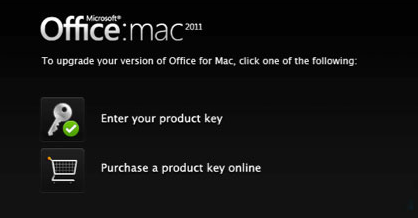
\includegraphics[width=3cm]{Images/faqshot_upgradefig4}
    \end{figure}

  \end{itemize}
 \end{frame}

 \begin{frame}{Why Ubuntu?}
  Convenience
   \begin{itemize}
   \pause
    \item 30,000+ packages/applications
   \pause
    \item Simple, yet intuitive and stylish UI
   \pause
    \item Integrated app store: Ubuntu Software Center
    \begin{figure}
     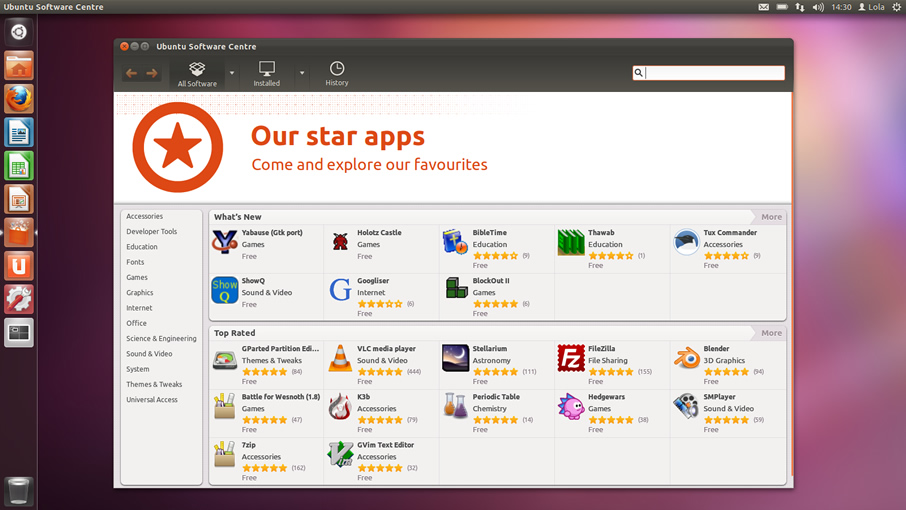
\includegraphics[width=5cm]{Images/softwarecentre_0}
    \end{figure}
   \pause
    \item Comprehensive software updates
   \pause
    \item Powerful shell: automation of tasks
   \end{itemize} 
 \end{frame}

 \begin{frame}{Why Ubuntu?}
  Secure
  \begin{itemize}
   \pause
   \item Multi-user operating system
   \pause
   \item Inherent design
   \pause
   \item No need of an anti-virus.
   \begin{figure}
    
\includegraphics[width=4cm]{Images/novirus}
   \end{figure}
   \pause
   \item No ports are opened by default.
   \pause
   \item Community support.
  \end{itemize}
 \end{frame}

 \begin{frame}{Why Ubuntu?}
  Speed/Performance
  \begin{itemize}
   \pause
   \item No clutter. No unwanted software. Light-weight.
   \pause
   \item Linux is the primary choice for mission-critical servers.
   \pause
   \item File systems like ext4, ZFS and UFS never need defragmentation
   \pause
   \item Designed for speed, stability, consistency and reliability
   \pause
   \item Quicker boot times
   \pause
   \item Infuse life into older computers
    \begin{figure}
     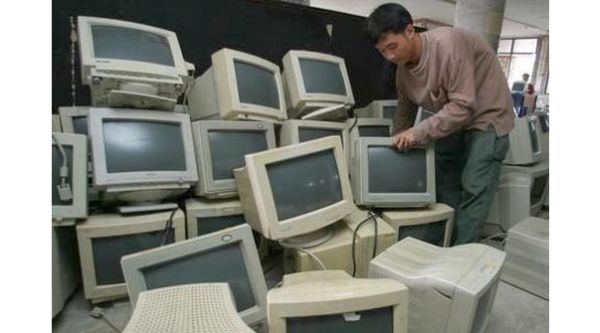
\includegraphics[width=5cm]{Images/old_desktop_computers}
    \end{figure}
  \end{itemize}
 \end{frame}
 
 \begin{frame}{Why Ubuntu?}
  \begin{itemize}
   \pause
   \item Productivity
    \begin{itemize}
     \item The Unity sidebar
     \item Virtual desktops
     \pause
    \end{itemize}
   \item Features are more closer to what users need.
  \end{itemize}
  \begin{figure}
   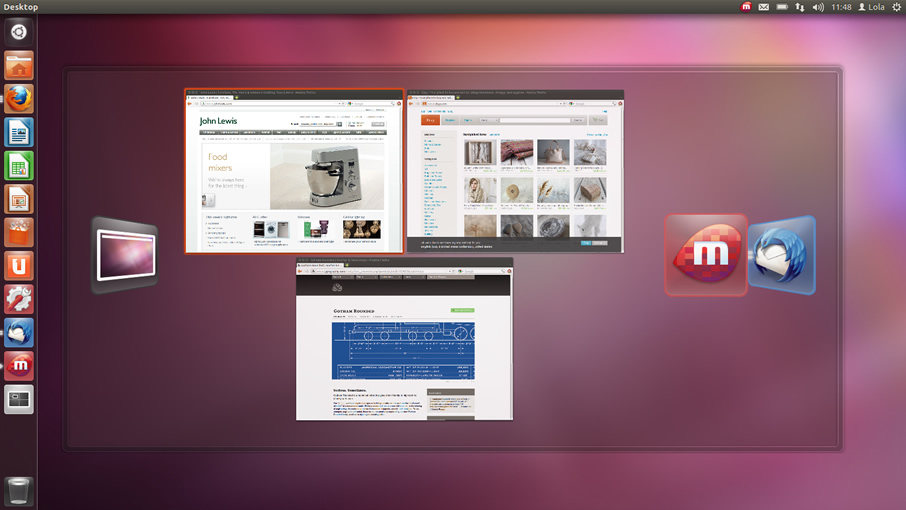
\includegraphics[width=7cm]{Images/altgrav}
  \end{figure}  
 \end{frame}

 \begin{frame}
  \begin{itemize}
   \item Fast installation
   \pause
   \item Software support
   \begin{itemize}
    \item
     \begin{figure}
      
\includegraphics[width=4cm]{Images/Open-Source-Applications-For-Cloud}
     \end{figure}
    \item Libreoffice X Microsoft Office
    \item Gimp X Adobe Photoshop
    \item Gcj X Java SDK
    \item Rhythmbox and Amarok X iTunes
   \end{itemize}
  \end{itemize}
 \end{frame}

 \begin{frame}{Why Ubuntu?}
  Stimulating
  \begin{itemize}
   \pause
   \item Open-source: freedom to tinker to your liking
   \pause
   \item No licensing issues: freedom to redistribute
   \pause
   \item Simpler/transparent design: everything is a file!
  \end{itemize}
 \end{frame}

 \begin{frame}
  \begin{itemize}
   \item A great accompaniment to students
   \pause
    \begin{itemize}
     \item The best way to learn unix, TCP/IP networking and computers in general
     \begin{figure}
      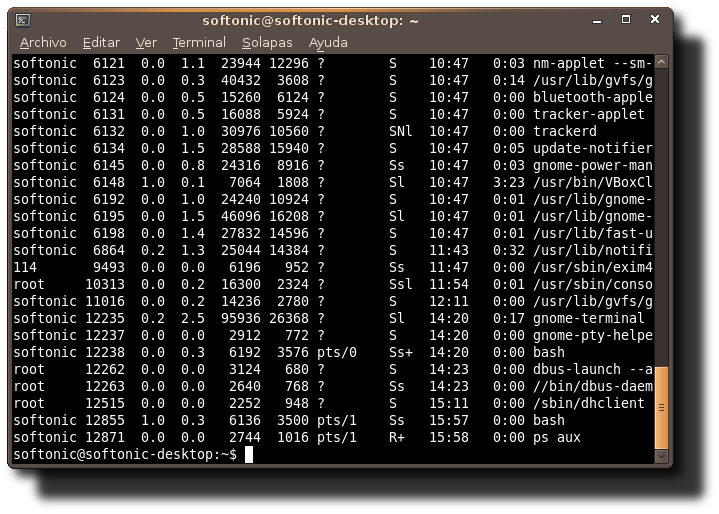
\includegraphics[width=5cm]{Images/linux_terminal}
     \end{figure}
     \pause
     \item Computing will be fun!
    \end{itemize}
  \end{itemize}
 \end{frame}

 \section{Benefits}
 \begin{frame}{Benefits}
  \begin{itemize}
   \pause
   \item Free, throughout its life --- Canonical
   \pause
   \item Assured six-month release cycle
   \pause
   \item Cut down licensing and maintenance costs
   \pause
   \item A great spurt in demand for UNIX/Linux sys admins and open-source developers.
   \pause
   \item Excellent community support.
  \end{itemize}
 \end{frame}

 \section{Who uses it?}
 \begin{frame}{Who uses it?}
  \begin{itemize}
   \pause
   \item Enterprises like Google, IBM, Facebook
   \pause
   \item PSUs like LIC
   \pause
   \item Kerala, Assam and Delhi govt.s
   \pause
   \item A lot of schools and colleges
  \end{itemize}
 \end{frame}

 \begin{frame}{How to go about using it?}
  \begin{itemize}
   \pause
   \item As the sole OS
   \pause
   \item Dual boot
  \end{itemize}
 \end{frame}

 \begin{frame}
  Virtual environment: Virtualbox, VMWare, Virtual PC
   \begin{figure}
    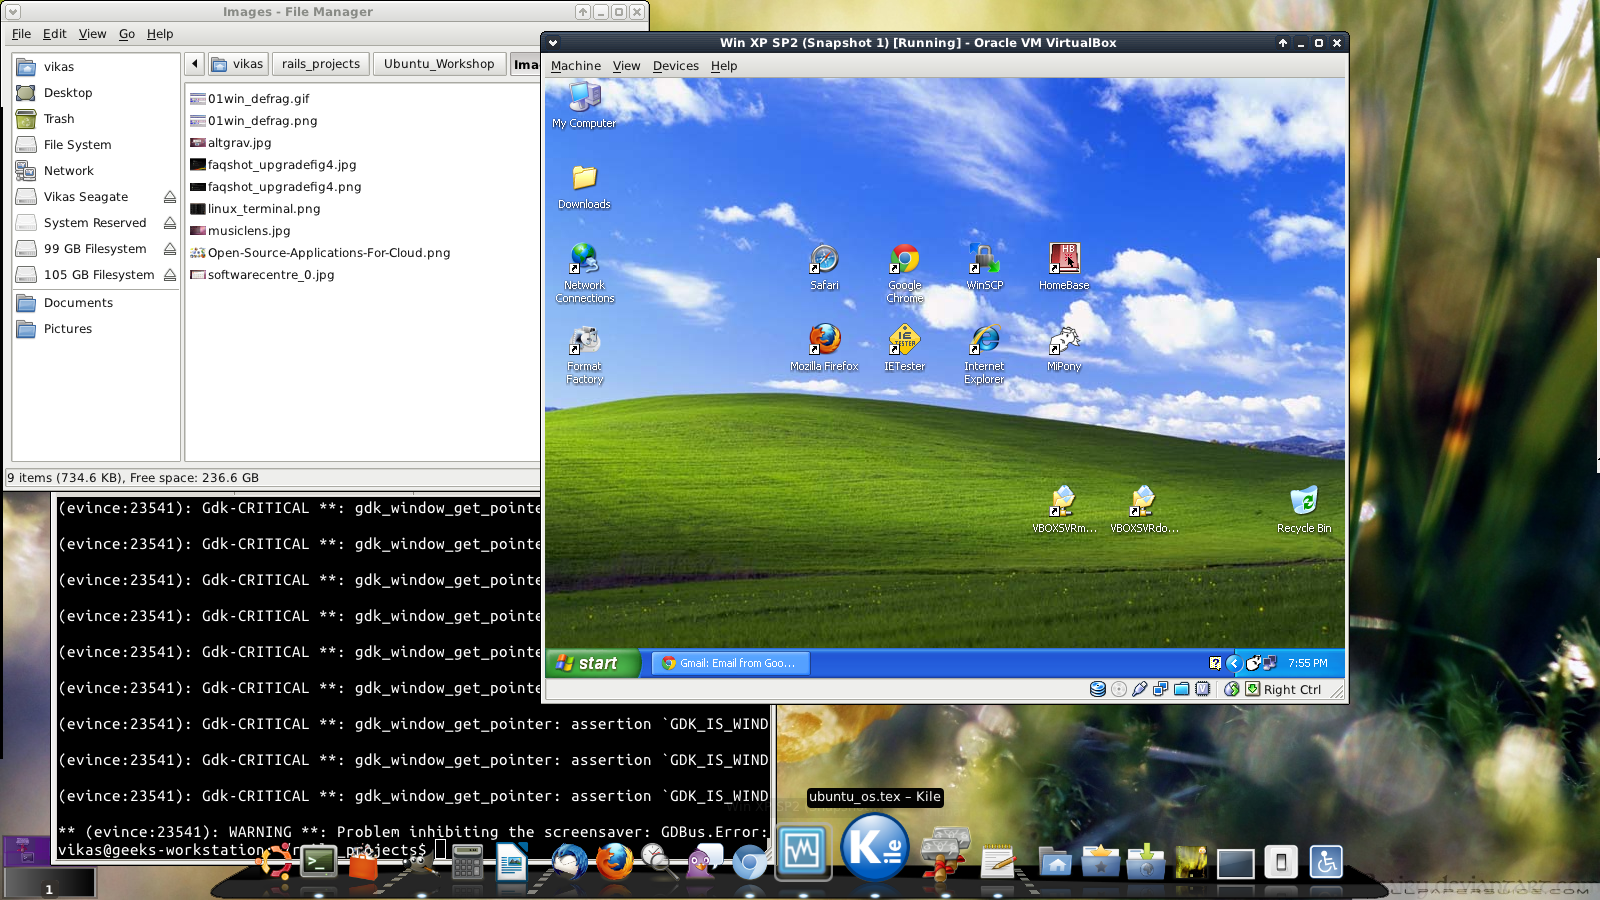
\includegraphics[width=8cm]{Images/virtualbox_screenshot}
   \end{figure}
 \end{frame}

 \section{What next?}
 \begin{frame}{What next?}
  \begin{itemize}
   \pause
   \item Rolling release Linux distros like Arch Linux and Gentoo
   \pause
   \item Customised installs across your laboratories. Custom kernels.
   \pause
   \item Thin client setups
    \begin{itemize}
     \item Zero maintenance
     \item Minimal infrastructural costs
     \item Greater control and censor
    \end{itemize}
   \pause
   \item Use it on servers
  \end{itemize}
 \end{frame}

 \begin{frame}{Thank you}
  \begin{center}
   \LARGE{Questions?}
  \end{center}
 \end{frame}


\end{document}
